

\documentclass[12pt, a4paper]{ article}
\usepackage[pdftex]{graphicx}
\usepackage{graphicx}

\setlength{\topmargin}{0in}
\setlength{\headheight}{0in}
\setlength{\headsep}{0in}
\setlength{\textheight}{9.5in}
\setlength{\textwidth}{6.5in}
\setlength{\oddsidemargin}{0in}
\setlength{\evensidemargin}{0in}


\date{}
\begin{document} 
\title{Blinky Lights - User Manual} 
\author{Kevin Yeap, Steven Morad, Connie Yu, Reid Anetsberger}
\maketitle 

% for comments use. 
% use this style for block comments
\iffalse
    This is a block comment.
    This line is also inside the block comment.
\fi

 %PAGE ===========================================================================================


\begin{center}

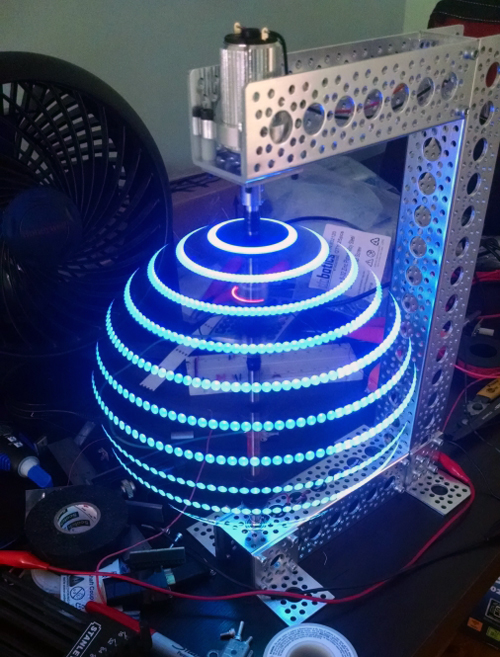
\includegraphics[]{C:/Users/KevinD/Documents/GitHub/blinkylights/doc/user_doc/b.PNG}

\end{center}






update this picture
\tableofcontents                       %this generates a table of contents automatically
\addcontentsline{toc}{section}{Table of Contents}





 %PAGE ===========================================================================================
\newpage
\addcontentsline{toc}{section}{Introduction}
\section*{Introduction:} 
\vspace{1cm}



THIS PAGE IS NOT DONE\\
intro to how Persistence of vision works to display patterns on the globe.\\\\

some hardware specs?\\
(how fast the LED blink)\\
(how fast the LED strip spins)\\
etc\\















%PAGE ===========================================================================================
\newpage
\addcontentsline{toc}{section}{Hardware Setup}
\section*{Hardware Setup:} 
\vspace{1cm}


\begin{center}
[INSERT SCREENSHOT OF  HARDWARE HERE]\\
I'd prefer that this picture be of the hardware when it is powered down and not spinning.
\end{center}


\vspace{1cm}
\noindent
1. Make sure no objects are obstructing the path of the LED strip. When the hardware is running the LED strip will be rotating at high speeds,  anything obstructing its path must be removed.\\\\
2. Plug in the AC adapter into a wall socket and the other end into the hardware.
\\\\
3. Turn on the hardware by flipping the power switch.
\\\\
WARNINGS: hardware spins at high speeds. Do not attempt to touch the hardware when it is spinning. 
Keep out of reach of children under 6 years of age. If you accidentally swallow hardware, seek professional help or contact a poison control center immediately.






 %PAGE ===========================================================================================
\newpage
\addcontentsline{toc}{section}{Bluetooth Setup}
\section*{Bluetooth Setup:} 
\vspace{1cm}

\begin{center}

\includegraphics[scale=0.75]{C:/Users/KevinD/Documents/GitHub/blinkylights/doc/user_doc/bluetooth.PNG}
\end{center}

\vspace{1cm}
\noindent
1. Turn on bluetooth on your pc and scan for surrounding devices.
\\\\
2. Connect to the device called "BLINKY LIGHTS"
\\\\
\begin{center}
[INSERT BLUETOOTH SCREENSHOT HERE]\\
screen shot of the computer detecting BLINKY LIGHTS
\end{center}

\vspace{1cm}
\noindent
3. Once your pc is connected to "BLINKY LIGHTS", execute the software.
\\\\










 %PAGE ===========================================================================================
\newpage
\addcontentsline{toc}{section}{Operating the Software}
\section*{Operating the Software:} 


\indent
\begin{center}
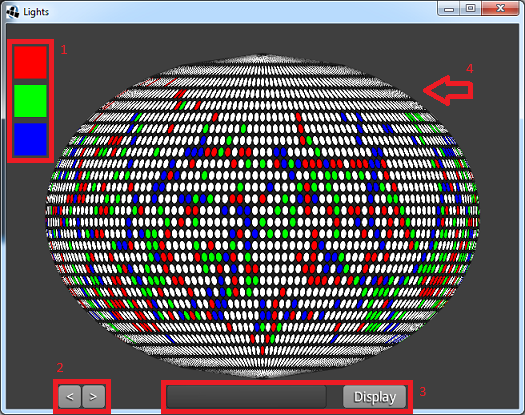
\includegraphics[scale=.8]{C:/Users/KevinD/Documents/GitHub/blinkylights/doc/user_doc/a_labels.PNG}
\end{center}


\noindent
\textbf{Software:} Execute the program. You should be greeted with the following GUI. Please read the corresponding number for a full explaination of the GUI.
\\\\\\
1. Click on a color to change the color of the brush. The color black is the eraser. 
\\\\
2. Click on an arrow to change the rotation of the globe canvas. Left arrow to rotate left. Right arrow to rotate right. Once an arrow is clicked the globe canvas will continuously rotate forever until the X button is pressed. The X button stops the globe canvas from rotating.
\\\\
3. For displaying text on the globe please see subsection b for more details.\textit{The globe canvas can only hold about 20 characters (including spaces)}
\\\\
4. Pressing the "clear" button sets all the LED pixels on the current layers to black. It clears all colors from the current layer.
\\\\\
5. Pressing the "Upload" button will upload the current pattern on the globe canvas and display it on the hardware.
\\\\
6. This is the globe canvas. This will be the canvas you will draw your patterns on. Please see subsection a for more details.
\vspace{5cm}





\newpage %-----------------------------------------------------------------------------------
\noindent \textit{Operating the Software (cont.)}

\addcontentsline{toc}{subsection}{a. Drawing on the Canvas}
\subsection*{a. Drawing on the Canvas:} 
\vspace{.5cm}

\noindent
1. Select a color to draw with by left-clicking a colored box off to the left. (Tutorial will use yellow)
\begin{center}
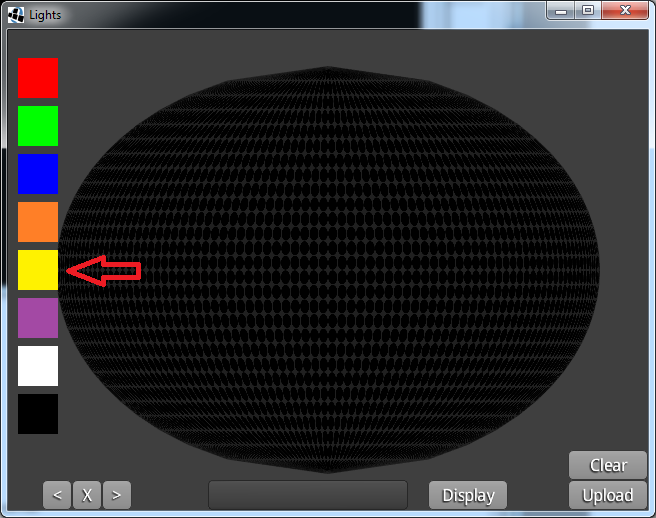
\includegraphics[scale=.65]{C:/Users/KevinD/Documents/GitHub/blinkylights/doc/user_doc/a_1.PNG}
\end{center}
\vspace{1cm}


\noindent
2. Left-click with your mouse on the globe canvas to fill in a "pixel". (chosen color was yellow for this example)
\begin{center}
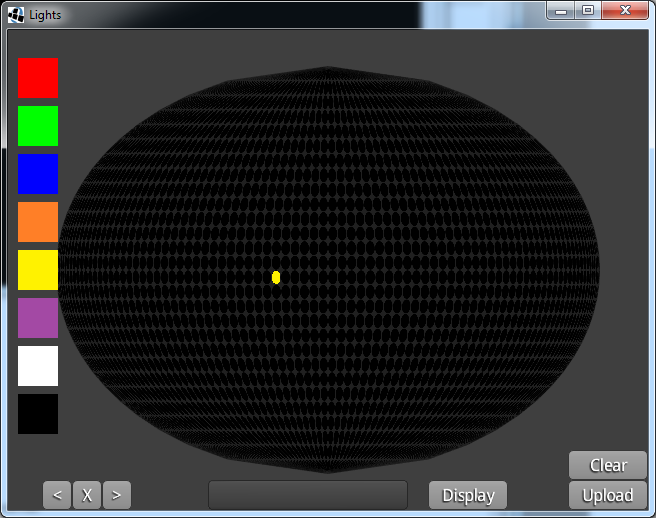
\includegraphics[scale=.65]{C:/Users/KevinD/Documents/GitHub/blinkylights/doc/user_doc/a_2.PNG}
\end{center}
\vspace{1cm}

\newpage %-----------------------------------------------------------------------------------
\noindent \textit{Operating the Software (cont.)}
\vspace{.5cm}


\noindent
3. pressing and holding the left mouse button allows you to drag your mouse over the cavas to fill in pixels that your mouse passses over. (chosen color was orange for this example)
\begin{center}
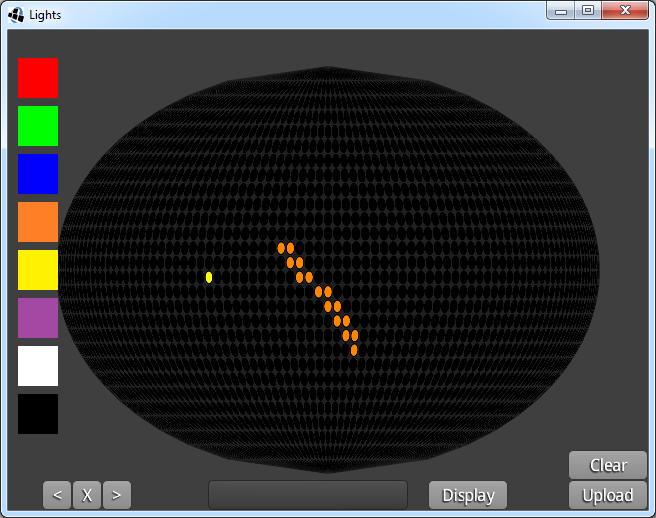
\includegraphics[scale=.65]{C:/Users/KevinD/Documents/GitHub/blinkylights/doc/user_doc/a_3.PNG}
\end{center}
\vspace{1cm}



\newpage %-----------------------------------------------------------------------------------
\noindent \textit{Operating the Software (cont.)}


\addcontentsline{toc}{subsection}{b. Displaying Text}
\subsection*{b. Displaying Text:} 
\vspace{.5cm}

\noindent
1. Type the characters that you want to display into the textbox.
\begin{center}
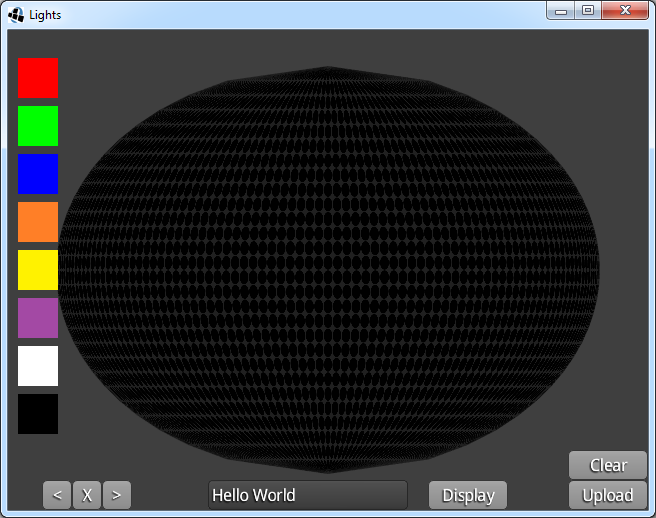
\includegraphics[scale=.65]{C:/Users/KevinD/Documents/GitHub/blinkylights/doc/user_doc/c_1.PNG}
\end{center}
\vspace{1cm}

\noindent
2. Click on the "Display" button to push the text onto the globe canvas.
\begin{center}
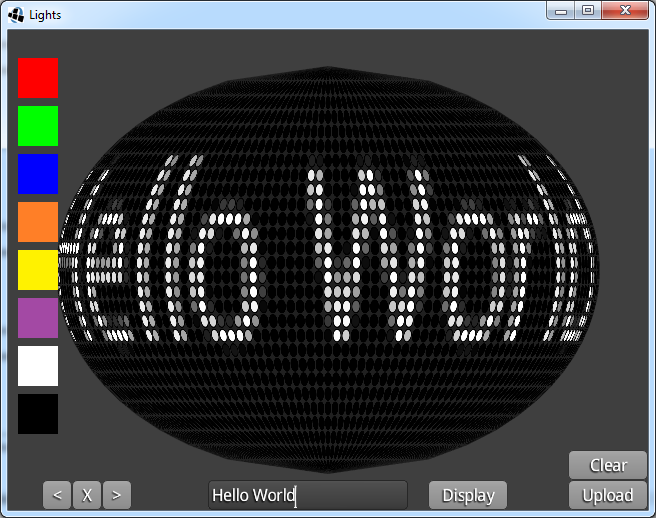
\includegraphics[scale=.65]{C:/Users/KevinD/Documents/GitHub/blinkylights/doc/user_doc/c_2.PNG}
\end{center}
\vspace{1cm}

















\end{document}